\documentclass{article}
\usepackage{amsmath, amssymb, tikz, multicol, tcolorbox, array, sfmath, enumerate, pgfplots}
\renewcommand{\familydefault}{\sfdefault}
\pgfplotsset{compat=newest}
\usetikzlibrary{arrows.meta}
\everymath{\displaystyle}
\tikzset{>=stealth}
\usepackage[top = 0.25in, bottom = 0.25in, left = 1in, right = 1in]{geometry}
\pagestyle{empty}
\raggedright

\newcounter{example}[section]
\newenvironment{example}[1][]{\refstepcounter{example}\par\medskip
   {\color{red}\textbf{Example~\theexample. #1}}}{\medskip}

\begin{document}

\section*{Graphs of Quadratic Functions}

\begin{tcolorbox}[colframe=orange!70!white, coltitle=black, title=\textbf{Summary}]
\begin{enumerate}
    \item Depending on how the graph is opening, the vertex is the minimum (or maximum) point on the graph.
    \item The axis of symmetry runs through the vertex and creates a mirrored image.
\end{enumerate}
\end{tcolorbox}

\subsection*{Vertex and Axis of Symmetry}

We will be looking at graphing equations in the form
\[ f(x) = ax^2 + bx + c \]
where $a$, $b$, and $c$ are real numbers with $a \neq 0$. 
\bigskip 


For $f(x)= x^2$, the graph below is a \textbf{parabola}.
\newline\\

\begin{center}
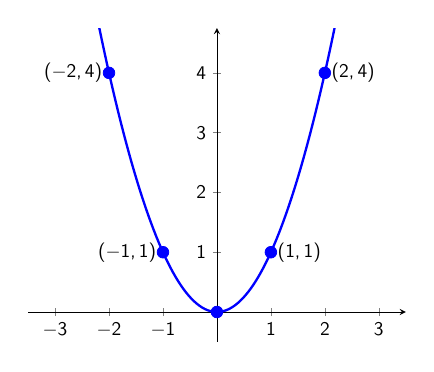
\begin{tikzpicture}[scale=0.7]
\begin{axis}[
axis lines = center,
xmin = -3.5, xmax = 3.5,
ymin = -0.5, ymax = 4.75,
xtick = {-3,-2,...,3},
ytick = {1,2,3,4}
]
\addplot[color=blue, very thick, samples=200, smooth] {x^2};
\addplot[color=blue, mark=*, only marks, mark size=3pt] coordinates {(-2,4) (-1,1) (0,0) (1,1) (2,4)};
\node at (axis cs:-2,4) [left] {$(-2,4)$};
\node at (axis cs:-1,1) [left] {$(-1,1)$};
% \node at (axis cs:0,0) [below] {$(0,0)$};
\node at (axis cs:1,1) [right] {$(1,1)$};
\node at (axis cs:2,4) [right] {$(2,4)$};
\end{axis}
\end{tikzpicture}
\end{center}
\bigskip 


The point $(0,0)$ is called the {\color{blue}\textbf{vertex}} of the parabola and can be either a minimum (smile) or maximum point (frown). 
\bigskip 

Through the vertex is a vertical line called the {\color{blue}\textbf{axis of symmetry}} that divides the parabola into 2 equal halves. 
\[
\text{Equation:} \quad x = x\text{-coordinate of the vertex}
\]

The {\color{blue}\textbf{zeros}} (a.k.a. the \textit{x-intercepts} or \textit{roots}) of a function are the values of $x$ \\ where the graph crosses the $x$-axis (a.k.a. $y = 0$); \underline{if it does at all}.
\bigskip 

\begin{example}
For each of the following:
\begin{itemize}
\item Find the coordinates of the vertex (use a graphing utility).
\item State whether the vertex is a maximum or minimum
\item Find the equation of the axis of symmetry
\item Find the zeros (if any)
\end{itemize}
\begin{multicols}{2}
\begin{enumerate}[(a)]
    \item $y = x^2 + 8x + 15$    
    \item $f(x) = -2x^2 + 11x - 12$
\end{enumerate}
\end{multicols}
\end{example}

\newpage 

% Let's examine the graph of $y = x^2 + 8x + 15$:

% \begin{minipage}{0.45\textwidth}
% \begin{tikzpicture}
% \begin{axis}
% [axis lines = middle, xmin = -6, xmax = 1, ymin = -2, ymax = 4, grid, xtick distance = 1, ytick distance = 1]
% \addplot[color = blue, thick, domain=-6:-2, samples=200] plot {x^2 + 8*x + 15};
% \addplot[color = blue, mark = *, only marks] coordinates {(-5,0) (-3,0)};
% \addplot[color = red, mark = diamond*, mark options = {scale = 1.5}, yshift=-0.1cm] coordinates {(-4,-1)};
% \end{axis}
% \end{tikzpicture}
% \end{minipage}
% \begin{minipage}{0.5\textwidth}
% \begin{itemize} \setlength{\itemsep}{20pt}
%     \item What do you get when you {\color{violet}\textbf{multiply}} the zeros of the function?
%     \item What do you get when you {\color{orange}\textbf{add}} the zeros of the function?
%     \item How does the $x$-coordinate of the vertex relate to the zeros?
%     \item How does $x^2 + 8x + 15$ factor?
% \end{itemize}
% \end{minipage}
% \vspace{1in} 

% Now, let's examine the graph of $f(x) = -2x^2 + 11x - 12$   \newline\\ 

% However, write it in the following way: $f(x) = -2\left(x^2 - \tfrac{11}{2}x + 6\right)$:

% \begin{minipage}{0.45\textwidth}
% \begin{tikzpicture}
% \begin{axis}
% [axis lines = middle, xmin = -1, xmax = 5, ymin = -2, ymax = 4, grid, xtick distance = 1, ytick distance = 1]
% \addplot[color = blue, thick, domain=1:5, samples=200] plot {-2*x^2 + 11*x - 12};
% \addplot[color = blue, mark = *, only marks] coordinates {(1.5,0) (4,0)};
% \addplot[color = red, mark = diamond*, mark options = {scale = 1.5}, yshift=0.1cm] coordinates {(2.75,3.125)};
% \end{axis}
% \end{tikzpicture}
% \end{minipage}
% \begin{minipage}{0.5\textwidth}
% \begin{itemize} \setlength{\itemsep}{24pt}
%     \item What do you get when you {\color{violet}\textbf{multiply}} the zeros of the function?
%     \item What do you get when you {\color{orange}\textbf{add}} the zeros of the function?
%     \item How does the $x$-coordinate of the vertex relate to the zeros?
% \end{itemize}
% \end{minipage}

% \vspace{2in}


\subsection*{General and Vertex Forms}

For a quadratic function: \newline 

\begin{minipage}{0.45\textwidth}
    \begin{itemize}
        \item The {\color{blue}\textbf{general form}} is $y = ax^2+bx+c$
        \begin{itemize}
            \item $a$, $b$, and $c$ are real numbers
            \item $a \neq 0$    
        \end{itemize} 
    \end{itemize}
\end{minipage}
\begin{minipage}{0.45\textwidth}
    \begin{itemize}
    \item The {\color{blue}\textbf{vertex form}} is $y = a(x-h)^2 + k$
    \begin{itemize}
        \item Vertex is $(h,k)$
        \item $a \neq 0$
        \item $a$, $h$, and $k$ are real numbers
    \end{itemize}
\end{itemize}
\end{minipage}
\vspace{0.5in}

To convert from general form $y = ax^2 + bx + c$ to standard form $y = a(x-h)^2+k$ 
\begin{enumerate}   
    \item Find the vertex:
    \begin{itemize} \setlength{\itemsep}{10pt}
        \item $x$-coordinate: $-\frac{b}{2a}$
        \item $y$-coordinate: Evaluate expression at $x$-coordinate
        \item \textbf{Or use graphing technology}
    \end{itemize}   
    \item Use the value of $a$ that is given.
\end{enumerate}
\bigskip 

\begin{example}
Write each of the following in vertex form.
\begin{enumerate}[(a)]
\begin{multicols}{3}
    \item $y = x^2 - 4x + 3$
    \item $y = 6 - x - x^2$
    \item $y = 3x^2 - 8x + 7$
\end{multicols}
\end{enumerate}
\end{example}
\vfill 

To convert from 
$y = a(x-h)^2 + k$	
form to 	
\[ y = ax^2 + bx + c\]
just {\color{violet}\textbf{do the math}} and remember your \underline{order of operations} (PEMDAS).
\bigskip 

\begin{example}
Convert each to general form.
\begin{enumerate}[(a)]
\begin{multicols}{3}
    \item $y = (x+2)^2 - 3$
    \item $y = -(x-7)^2 + 10$
    \item $y = 4\left(x-1\right)^2 + 1$
\end{multicols}
\end{enumerate}
\end{example}

\vfill 

\end{document}
